%iffalse
\let\negmedspace\undefined
\let\negthickspace\undefined
\documentclass[journal,12pt,onecolumn]{IEEEtran}
\usepackage{cite}
\usepackage{amsmath,amssymb,amsfonts,amsthm}
\usepackage{algorithmic}
\usepackage{graphicx}
\usepackage{textcomp}
\usepackage{xcolor}
\usepackage{txfonts}
\usepackage{listings}
\usepackage{enumitem}
\usepackage{mathtools}
\usepackage{gensymb}
\usepackage{comment}
\usepackage[breaklinks=true]{hyperref}
\usepackage{tkz-euclide} 
\usepackage{listings}
\usepackage{gvv}                                        
% \usepackage{gvv}  
\usepackage[latin1] {inputenc}
\usepackage{xparse}
\usepackage{color}                                            
\usepackage{array}                                            
\usepackage{longtable}                                       
\usepackage{calc}                                             
\usepackage{multirow}
\usepackage{multicol}
\usepackage{hhline}                                           
\usepackage{ifthen}                                           
\usepackage{lscape}
\usepackage{tabularx}
\usepackage{array}
\usepackage{float}
\newtheorem{theorem}{Theorem}[section]
\newtheorem{problem}{Problem}
\newtheorem{proposition}{Proposition}[section]
\newtheorem{lemma}{Lemma}[section]
\newtheorem{corollary}[theorem]{Corollary}
\newtheorem{example}{Example}[section]
\newtheorem{definition}[problem]{Definition}
\newcommand{\BEQA}{\begin{eqnarray}}
\newcommand{\EEQA}{\end{eqnarray}}
\usepackage{float}
%\newcommand{\define}{\stackrel{\triangle}{=}}
\theoremstyle{remark}
%\newtheorem{rem}{Remark}
% Marks the beginning of the document
\begin{document}
\title{GATE BT 2025}
\author{EE25BTECH11044 - Pappula Sai Hasini}
\maketitle
\renewcommand{\thefigure}{\theenumi}
\renewcommand{\thetable}{\theenumi}
%GATE BT 2025

\begin{enumerate}


\item Is there any good show television tonight? Select the most appropriate option to complete the above sentence.
\begin{multicols}{2}
\begin{enumerate}
\item in
\item at
\item within
\item on
\end{enumerate}
\end{multicols}
\hfill (GATE BT 2025)

\item As the police officer was found guilty of embezzlement, he was dismissed from the service in accordance with the Service Rules. Select the most appropriate option to complete the above sentence.
\begin{multicols}{2}
\begin{enumerate}
\item sumptuously
\item brazenly
\item unintentionally
\item summarily
\end{enumerate}
\end{multicols}
\hfill (GATE BT 2025)

\item The sum of the following infinite series is:
\[
\frac{1}{1!} + \frac{1}{2!} + \frac{1}{3!} + \frac{1}{4!} + \frac{1}{5!} + \cdots
\]
\begin{multicols}{2}
\begin{enumerate}
\item $\pi$
\item $1 + e$
\item $e - 1$
\item $e$
\end{enumerate}
\end{multicols}
\hfill (GATE BT 2025)

\item A thin wire is used to construct all the edges of a cube of $1 \, \text{m}$ side by bending, cutting and soldering the wire. If the wire is $12 \, \text{m}$ long, what is the minimum number of cuts required to construct the wire frame to form the cube?
\begin{multicols}{2}
\begin{enumerate}
\item $3$
\item $4$
\item $6$
\item $12$
\end{enumerate}
\end{multicols}
\hfill (GATE BT 2025)

\item The figures $I$, $II$ and $III$ are parts of a sequence. Which one of the following options comes next in the sequence at $IV$?

\begin{figure}
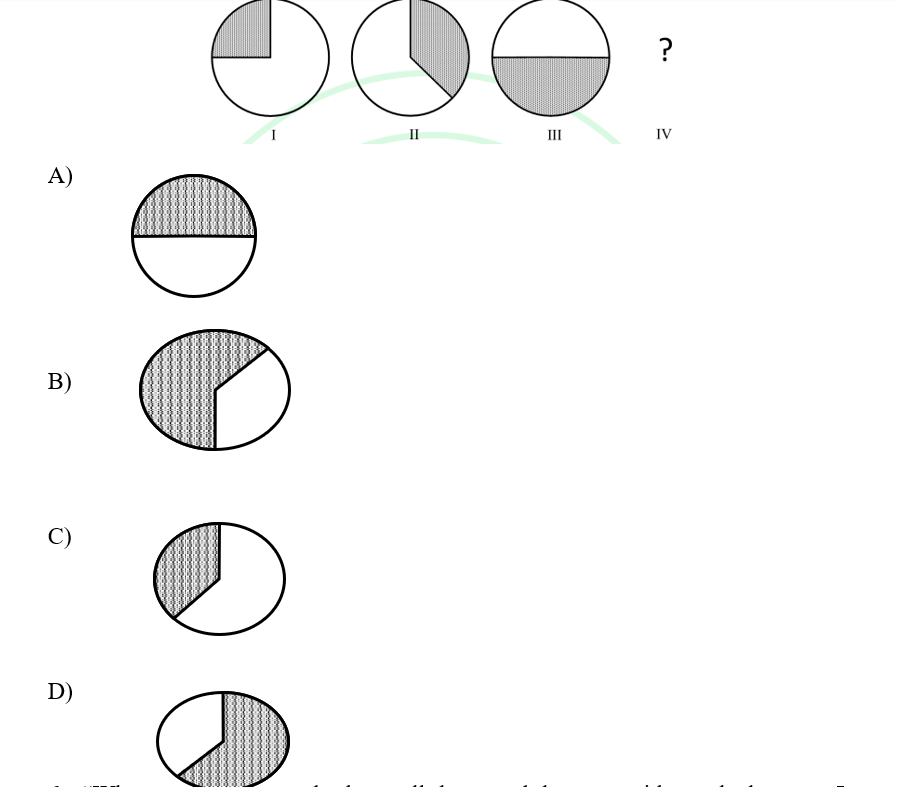
\includegraphics[width=\columnwidth]{figs/sequence.png}
\end{figure}

\begin{enumerate}
\item Option A
\item Option B
\item Option C
\item Option D
\end{enumerate}
\hfill (GATE BT 2025)

\item Why do they pull down and do away with crooked streets, I wonder, which are my delight, and hurt no man living? Every day the wealthier nations are pulling down one or another in their capitals and their great towns: they do not know why they do it; neither do I. It ought to be enough, surely, to drive the great broad ways which commerce needs and which are the life-channels of a modern city, without destroying all history and all the humanity in between: the islands of the past. 

(From Hilaire Bellocs The Crooked Streets)

Based only on the information provided in the above passage, which one of the following statements is true?
\begin{enumerate}
\item The author of the passage takes delight in wondering.
\item The wealthier nations are pulling down the crooked streets in their capitals.
\item In the past, crooked streets were only built on islands.
\item Great broad ways are needed to protect commerce and history.
\end{enumerate}
\hfill (GATE BT 2025)

\item Rohit goes to a restaurant for lunch at about 1 PM. When he enters the restaurant, he notices that the hour and minute hands on the wall clock are exactly coinciding. After about an hour, when he leaves the restaurant, he notices that the clock hands are again exactly coinciding. How much time (in minutes) did Rohit spend at the restaurant?  
\begin{multicols}{2}
\begin{enumerate}
    \item $64 \frac{6}{11}$
    \item $66 \frac{5}{13}$
    \item $65 \frac{5}{11}$
    \item $66 \frac{6}{13}$
\end{enumerate} 
\end{multicols}
\hfill (GATE BT 2025)

\item A color model is shown in the figure with color codes: Yellow (Y), Magenta (M), Cyan (Cy), Red (R), Blue (Bl), Green (G), and Black (K).  
Which one of the following options displays the color codes that are consistent with the color model?  

\begin{figure}
    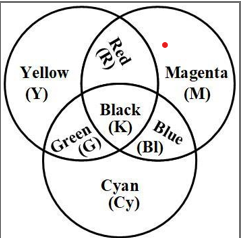
\includegraphics[width=0.6\columnwidth]{figs/question.png}
\end{figure}

\begin{enumerate}
    \item 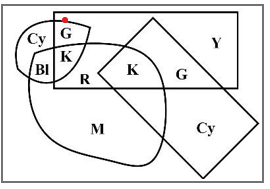
\includegraphics[width=0.6\columnwidth]{figs/option1.png}
    \item 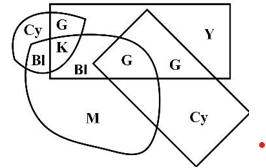
\includegraphics[width=0.6\columnwidth]{figs/option2.png}
    \item 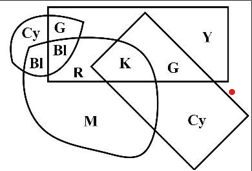
\includegraphics[width=0.6\columnwidth]{figs/option3.png}
    \item 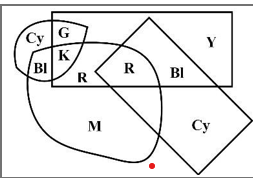
\includegraphics[width=0.6\columnwidth]{figs/option4.png}
\end{enumerate}

\hfill (GATE BT 2025)

\item A circle with center at $(x, y) = (0.5, 0)$ and radius $0.5$ intersects with another circle with center at $(x, y) = (1, 1)$ and radius $1$ at two points. One of the points of intersection $(x, y)$ is:  
\begin{multicols}{2}

\begin{enumerate}
    \item $(0, 0)$
    \item $(0.2, 0.4)$
    \item $(0.5, 0.5)$
    \item $(1, 2)$
\end{enumerate} 
\end{multicols}
\hfill (GATE BT 2025)

\item Kochs postulate was established by Robert Koch while working on a disease caused by  
\begin{multicols}{2}
\begin{enumerate}
    \item Mycobacterium tuberculosis
    \item Bacillus anthracis
    \item Streptococcus pneumoniae
    \item Bacillus subtilis
\end{enumerate}  
\end{multicols}
\hfill (GATE BT 2025)

\item An object is said to have an $n$-fold rotational symmetry if the object, rotated by an angle of $\dfrac{2\pi}{n}$, is identical to the original. Which one of the following objects exhibits 4-fold rotational symmetry about an axis perpendicular to the plane of the screen? {Note: The figures shown are representative.}

\begin{enumerate}
    \item 
\includegraphics[width=0.3\columnwidth]{figs/opt1.png}
    \item 
\includegraphics[width=0.3\columnwidth]{figs/opt2.png}
    \item 
\includegraphics[width=0.3\columnwidth]{figs/opt3.png}
    \item 
\includegraphics[width=0.3\columnwidth]{figs/opt4.png}
\end{enumerate}

\hfill (GATE BT 2025)


\item Corynebacterium diphtheriae causes diphtheria in humans, only when this bacterium is infected by  
\begin{multicols}{2}
\begin{enumerate}
    \item phage $\beta$
    \item epsilon phage
    \item T4 phage
    \item lambda phage
\end{enumerate}  
\end{multicols}
\hfill (GATE BT 2025)

\item Let $y(t)$ be a bacterial population whose growth is given by  
\[
\frac{dy}{dt} = \lambda (y + 2)
\]  
where $\lambda$ is the growth rate constant. If $y(0) = 1$ and $y(1) = 4$, then the value of $\lambda$ is  
\begin{multicols}{2}
\begin{enumerate}
    \item $\ln 2$
    \item $\ln 3$
    \item $\ln 4$
    \item $\ln 6$
\end{enumerate}
\end{multicols}
\hfill (GATE BT 2025)

\item The minimum value of the function  
\[
f(x) = x + \frac{4}{x} 
\]  
is  
\begin{multicols}{2}
\begin{enumerate}
    \item $1$
    \item $2$
    \item $3$
    \item $4$
\end{enumerate}
\end{multicols}
\hfill (GATE BT 2025)

\item The diversity in T-cell receptors is generated by  

\begin{enumerate}
    \item gene rearrangements
    \item somatic hypermutation of rearranged V region
    \item gene conversion
    \item class switching
\end{enumerate}  
\hfill (GATE BT 2025)

\item Which one of the following is true for piRNAs?  

\begin{enumerate}
    \item piRNAs silence transposable elements in germ cells
    \item piRNA is the abbreviation of P-element interacting RNA
    \item piRNAs modify the $2'$-OH of ribose with methyl group
    \item piRNA is a long non-coding RNA
\end{enumerate}  
\hfill (GATE BT 2025)

\item Which one of the following coenzymes is utilised by alanine racemase for the conversion of L-Alanine to D-Alanine?  
\begin{multicols}{2}
\begin{enumerate}
    \item Pyridoxal phosphate
    \item Thiamine pyrophosphate
    \item Tetrahydrofolate
    \item Flavin mononucleotide
\end{enumerate}  
\end{multicols}
\hfill (GATE BT 2025)

\item Correctly match the following Monosaccharides with their respective Epimers.  

\begin{tabular}{ll}
Monosaccharide & Epimer \\
P. D-mannose & 1. C-3 epimer of D-glucose \\
Q. D-allose & 2. C-4 epimer of D-glucose \\
R. D-galactose & 3. C-4 epimer of D-mannose \\
S. D-talose & 4. C-2 epimer of D-glucose \\
 & 5. C-5 epimer of D-glucose
\end{tabular}  

\begin{enumerate}
    \item P-4; Q-1; R-2; S-3
    \item P-5; Q-1; R-2; S-3
    \item P-4; Q-3; R-5; S-1
    \item P-1; Q-5; R-3; S-2
\end{enumerate}  
\hfill (GATE BT 2025)

\item Correctly match the following Product classes with their representative Products  

\begin{tabular}{ll}
Product class & Product \\
P. Biofuel & 1. Cellulose \\
Q. Bioplastic & 2. Cephalosporin \\
R. Industrial enzyme & 3. Butanol \\
S. Antibiotic & 4. Poly-lactic acid \\
 & 5. Rituximab
\end{tabular}  

\begin{enumerate}
    \item P-1; Q-5; R-3; S-2
    \item P-3; Q-4; R-5; S-2
    \item P-3; Q-2; R-1; S-5
    \item P-3; Q-4; R-1; S-2
\end{enumerate}  
\hfill (GATE BT 2025)

\item Which one of the following hosts is used in mammalian cell culture for the production of glycosylated recombinant therapeutic proteins?  
\begin{multicols}{2}
\begin{enumerate}
    \item Pichia pastoris
    \item Sf9 cells
    \item Escherichia coli
    \item Chinese hamster ovary cells
\end{enumerate}  
\end{multicols}
\hfill (GATE BT 2025)

\item Which of the following features is/are used to distinguish Archaea from Bacteria?  
\begin{multicols}{2}
\begin{enumerate}
    \item Gram-staining
    \item Peptidoglycan in the cell wall
    \item Presence of N-acetylglucosamine
    \item 16S rRNA sequences
\end{enumerate}  
\end{multicols}
\hfill (GATE BT 2025)

\item Which of the following enzymes is/are involved in the biogenesis of miRNA?  
\begin{multicols}{2}
\begin{enumerate}
    \item Drosha
    \item Cas9
    \item XRCC4
    \item Dicer
\end{enumerate}  
\end{multicols}
\hfill (GATE BT 2025)

\item Which of the following separation processes is/are based on molecular size?  
\begin{multicols}{2}
\begin{enumerate}
    \item Size-exclusion chromatography
    \item Ion exchange chromatography
    \item Membrane ultrafiltration
    \item Ultracentrifugation
\end{enumerate}  
\end{multicols}
\hfill (GATE BT 2025)
\item Which of the following show(s) optical activity at $100$ mM concentration in water?  
\begin{multicols}{2}
\begin{enumerate}
    \item Solution of NaCl
    \item Solution of D-Glucose
    \item Solution of Glycine
    \item Solution of L-Proline
\end{enumerate}  
\end{multicols}
\hfill (GATE BT 2025)

\item Which of the following fluids exhibit(s) non-Newtonian behaviour at 25 $^\circ$C?  
\begin{multicols}{2}
\begin{enumerate}
    \item Toothpaste
    \item Mercury
    \item Brine
    \item Blood plasma
\end{enumerate}  
\end{multicols}
\hfill (GATE BT 2025)

\item Which of the following compounds have the same degree of reduction per carbon-mole?  
\begin{multicols}{2}
\begin{enumerate}
    \item Glucose
    \item Lactic acid
    \item Acetic acid
    \item Formic acid
\end{enumerate}  
\end{multicols}
\hfill (GATE BT 2025)

\item A recombinant protein is secreted extracellularly in soluble form by an E. coli culture. Which of the following downstream processes is/are involved in the purification of the extracellular secreted protein?  
\begin{multicols}{2}
\begin{enumerate}
    \item Cell disruption
    \item Membrane ultrafiltration
    \item Solubilisation of inclusion bodies
    \item Liquid chromatography
\end{enumerate}  
\end{multicols}
\hfill (GATE BT 2025)

\item If the doubling time of a bacterial population is 3 hours, then its average specific growth rate during this period is h$^{-1}$.  
(Round off to two decimal places)  
\hfill (GATE BT 2025)

\item For a mechanically reversible isobaric process taking place in a closed system involving 5 moles of an ideal gas, the temperature increases from an initial value of 300 K to a final value of 450 K. If the specific heat capacity at constant volume ($C_v$) is given as 12.5 J mol$^{-1}$ K$^{-1}$ and gas constant is 8.314 J mol$^{-1}$ K$^{-1}$, the amount of heat transferred to the system will be \_\_\_J.  
\hfill (GATE BT 2025)

\item The allele associated with albinism in humans is recessive ($c$). The probability that an albino male ($cc$) and a carrier female ($Cc$) will have an offspring with normal skin pigmentation is \_\_\_.  
(Round off to one decimal place)  
\hfill (GATE BT 2025)

\item The contour length of a B-DNA molecule that encodes a bacterial protein of 33 kDa is \_\_\_ nm.  
\hfill (GATE BT 2025)

\item Within the Michaelis-Menten framework, the ratio of $v_0 / V_{\max}$ when $[S] = 20 \times K_m$ is .  
(Round off to two decimal places)  
\hfill (GATE BT 2025)

\item Consider a nonlinear algebraic equation, $e^x - 2 = 0$. Using the Newton-Raphson method, with the initial guess of $x_0 = 1$, the approximated value of the root of the equation after one iteration is \_\_\_.  
(Round off to two decimal places)  
\hfill (GATE BT 2025)

\item The value of $k$, for which the linear equations $2x + 3y = 6$ and $4x + 6y = 3k$ have at least one solution, is \_\_\_.  
(Answer in integer)  
\hfill (GATE BT 2025)

\item Two fair six-sided dice, with sides numbered 1 to 6, are thrown once. The probability of getting 7 as the sum of the numbers on the top side of the dice is \_\_\_.  
(Round off to two decimal places)  
\hfill (GATE BT 2025)

\item Correctly match the Microorganisms with their respective Nutrition and energy requirement.  

\begin{tabular}{ll}
Microorganisms & Nutrition and energy requirement \\
P. Photolithoautotrophs & 1. Use organic compounds as a source of energy, hydrogen, electron and carbon \\
Q. Chemoorganoheterotrophs & 2. Use light energy and use CO$_2$ as their carbon source \\
R. Chemolithoautotrophs & 3. Use light energy and use organic compounds as electron donor and carbon source \\
S. Photoorganoheterotrophs & 4. Oxidise reduced-inorganic molecules as energy and electron source but derive carbon from organic sources
\end{tabular}  

\begin{enumerate}
    \item P-2; Q-1; R-4; S-3
    \item P-2; Q-1; R-3; S-4
    \item P-1; Q-2; R-4; S-3
    \item P-4; Q-1; R-2; S-3
\end{enumerate}  
\hfill (GATE BT 2025)

\item Correctly match the Inhibitor with its respective Function in mitochondrial respiration.  

\begin{tabular}{ll}
Inhibitor & Function \\
P. FCCP & 1. Inhibits cytochrome c oxidase \\
Q. Cyanide & 2. Makes the membrane permeable to protons \\
R. Oligomycin A & 3. Blocks mitochondrial uptake of succinate \\
S. Butyl malonate & 4. Inhibits ATP synthase
\end{tabular}  

\begin{enumerate}
    \item P-2; Q-1; R-4; S-3
    \item P-2; Q-3; R-1; S-4
    \item P-2; Q-4; R-3; S-1
    \item P-3; Q-1; R-2; S-4
\end{enumerate}  
\hfill (GATE BT 2025)


\item An octapeptide composed of these L-amino acids: Lys, Thr, Ser, Met, Arg, Trp, Tyr, Glu, was subjected to analyses with the following outcomes:  
\hfill (GATE BT 2025)


P. The N-terminal sequencing analysis by Sangers method yielded Ser at the N-terminus  
Q. Chymotrypsin treatment gave a pentapeptide, a 
Tyr containing dipeptide and a free Glu  
R. Cyanogen bromide treatment gave two tetrapeptides  
S. Trypsin treatment gave two tripeptides and a dipeptide  

Which one of the following is the correct octapeptide sequence?  

\begin{enumerate}
    \item Ser-Tyr-Arg-Met-Lys-Thr-Trp-Glu
    \item Ser-Arg-Lys-Met-Tyr-Thr-Trp-Glu
    \item Ser-Met-Lys-Arg-Thr-Tyr-Trp-Glu
    \item Ser-Arg-Met-Lys-Trp-Thr-Tyr-Glu
\end{enumerate}  
\hfill (GATE BT 2025)

\item Correctly match the type of Hypersensitivity reaction with its respective Example.  

\begin{tabular}{ll}
Hypersensitivity reaction & Example \\
P. Type I & 1. Tuberculin reaction \\
Q. Type II & 2. Arthus reaction \\
R. Type III & 3. Chronic urticaria \\
S. Type IV & 4. Systemic anaphylaxis
\end{tabular}  

\begin{enumerate}
    \item P-3; Q-4; R-2; S-1
    \item P-4; Q-3; R-1; S-2
    \item P-4; Q-3; R-2; S-1
    \item P-2; Q-3; R-4; S-1
\end{enumerate}  
\hfill (GATE BT 2025)

\item Correctly match the Enzyme with its respective Function.  

\begin{tabular}{ll}
Enzyme & Function \\
P. Gyrase & 1. Removes a damaged base by cleaving the bond between sugar and base \\
Q. Deadenylase & 2. Provides a swivel allowing one DNA strand to rotate around the other \\
R. Glycosylase & 3. Catalyses bond formation between 3-OH and 5-phosphate end of nucleotides in duplex DNA \\
S. DNA ligase & 4. Is an exoribonuclease that removes the poly(A) tail
\end{tabular}  

\begin{enumerate}
    \item P-2; Q-4; R-1; S-3
    \item P-1; Q-4; R-2; S-3
    \item P-2; Q-1; R-4; S-3
    \item P-3; Q-2; R-1; S-4
\end{enumerate}  
\hfill (GATE BT 2025)

\item Correctly match the Coenzyme with its respective involvement in a specific Reaction type.\\

Coenzyme \hspace{1cm} Reaction type \\
P. Thiamine pyrophosphate \hspace{0.5cm} 1. Acyl group transfer \\
Q. Tetrahydrofolate \hspace{1.3cm} 2. Transfer of one carbon group \\
R. Flavin adenine dinucleotide \hspace{0.3cm} 3. Transfer of methyl group \\
S. 5-Deoxyadenosyl cobalamin \hspace{0.3cm} 4. Oxidation-reduction \\
\hspace{3cm} 5. Aldehyde transfer

\begin{enumerate}
    \item P-5; Q-2; R-4; S-3
    \item P-5; Q-1; R-2; S-3
    \item P-1; Q-2; R-4; S-5
    \item P-5; Q-3; R-1; S-2
\end{enumerate}
\hfill (GATE BT 2025)

\item A thermometer measuring body temperature follows a first-order response with a time constant of $40$ seconds. The instrument will reach $95\%$ of its steady-state output at $~$ seconds. (Round off to the nearest integer)
\begin{multicols}{2}
\begin{enumerate}
    \item $60$
    \item $80$
    \item $120$
    \item $160$
\end{enumerate}
\end{multicols}
\hfill (GATE BT 2025)

\item The output $y(t)$ of a first-order process is governed by the following differential equation:
\[
\frac{dy}{\tau_p \, dt} + y = K_p f(t)
\]
where $\tau_p$ is a non-zero time constant, $K_p$ is the gain, and $f(t)$ is the input with $f(0) = 0$. Assume $y(0) = 0$. The transfer function for this process is (consider $s$ as the independent variable in the Laplace domain)

\begin{enumerate}
    \item $\frac{K_p}{\tau_p s + 1}$
    \item $\frac{\tau_p}{K_p s + 1}$
    \item $\frac{\tau_p}{K_p (s + 1)}$
    \item $\frac{K_p}{\tau_p (s + 1)}$
\end{enumerate}
\hfill (GATE BT 2025)

\item For a specific bioreactor configuration, the power requirement for a Rushton-turbine impeller agitating an unaerated Newtonian fluid in the turbulent regime will be

\begin{enumerate}
    \item proportional to the stirring speed of the impeller
    \item proportional to the square of the stirring speed of the impeller
    \item proportional to the cube of the stirring speed of the impeller
    \item inversely proportional to the stirring speed of the impeller
\end{enumerate}
\hfill (GATE BT 2025)

\item Let $m$ and $n$ be fixed real numbers. If the function $y(t) = C_1 e^t + C_2 e^{-t}$ is a solution of
\[
\frac{d^2 y}{dt^2} + m \frac{dy}{dt} + n y = 0
\]
for any constants $C_1$ and $C_2$, then $m + n$ is equal to
\begin{multicols}{2}
\begin{enumerate}
    \item $-2$
    \item $-1$
    \item $0$
    \item $1$
\end{enumerate}
\end{multicols}
\hfill (GATE BT 2025)

\item If the function
\[
f(x) = 
\begin{cases} 
\sin 2x, & x > 0, \\
a + b x, & x \le 0,
\end{cases}
\]
where $a$ and $b$ are constants, is differentiable at $x = 0$, then $a + b$ is equal to
\begin{multicols}{2}
\begin{enumerate}
    \item $0$
    \item $1$
    \item $2$
    \item $3$
\end{enumerate}
\end{multicols}
\hfill (GATE BT 2025)

\item Correctly match the following Bioinformatic tool/Database with its respective Utility.\\

Bioinformatic tool/Database \hspace{1cm} Utility \\
P. BLAST \hspace{1cm} 1. Database for 3D protein structures \\
Q. Bowtie \hspace{1cm} 2. Tool to identify similarity of a query sequence to existing sequences available in databanks \\
R. AlphaFold \hspace{1cm} 3. Tool to align short read DNA sequences obtained from Next-generation sequencing to a reference genome \\
S. PDB \hspace{1cm} 4. AI tool to predict protein structures

\begin{enumerate}
    \item P-2; Q-3; R-1; S-4
    \item P-2; Q-3; R-4; S-1
    \item P-3; Q-2; R-4; S-1
    \item P-4; Q-1; R-2; S-3
\end{enumerate}
\hfill (GATE BT 2025)

\item Correctly match the herbicide with its mode of development of resistance in plants.\\

Herbicide \hspace{1cm} Mode of development of resistance \\
P. Imidazolinones \hspace{0.5cm} 1. Transformation of bacterial nitrilase gene \\
Q. Bromoxynil \hspace{1.3cm} 2. Transformation of resistant version of acetolactate synthetase \\
R. Glufosinate \hspace{1.3cm} 3. Transformation of tfdA gene from Alcaligenes, which encodes a dioxygenase \\
\hspace{3cm} 4. Transformation of bar gene from Streptomyces hygroscopicus which encodes phosphinothricin acetyltransferase

\begin{enumerate}
    \item P-2; Q-1; R-4
    \item P-2; Q-1; R-3
    \item P-1; Q-2; R-3
    \item P-4; Q-1; R-3
\end{enumerate}
\hfill (GATE BT 2025)

\item Which of the following statements is/are true regarding the effect of the concentration of metabolic intermediates on glycolysis in erythrocytes?

\begin{enumerate}
    \item Increased $AMP$ levels stimulate glycolysis
    \item Increased $citrate$ inhibits glycolysis
    \item Increased $glucose\ 6\!-\!phosphate$ inhibits glycolysis
    \item Increased $fructose\ 1,6\!-\!bisphosphate$ stimulates glycolysis
\end{enumerate}
\hfill (GATE BT 2025)

\item Which of the following statements about initiation of DNA replication in eukaryotes is/are true?

\begin{enumerate}
    \item DNA replication is initiated at the origin of replication licensed by loading of $Mcm$ helicase complex
    \item Loading of $Mcm$ helicase complex takes place in $S$ phase
    \item $Mcm$ helicase complex are activated by $S$-$Cdks$
    \item $Mcm$ helicase complex is responsible for loading of origin recognition complex
\end{enumerate}
\hfill (GATE BT 2025)

\item Which of the following proteins is/are involved in intraflagellar transport?
\begin{multicols}{2}
\begin{enumerate}
    \item $Microtubules$
    \item $Myosin$
    \item $Actin$
    \item $Kinesin$
\end{enumerate}
\end{multicols}
\hfill (GATE BT 2025)

\item Which of the following statements is/are true about telomerase?

\begin{enumerate}
    \item Telomerase has $5'\!-\!3'$ DNA-dependent DNA polymerisation activity
    \item Telomerase has $5'\!-\!3'$ RNA-dependent DNA polymerisation activity
    \item Telomerase contains an RNA subunit
    \item Telomerase has $3'\!-\!5'$ DNA-dependent DNA polymerisation activity
\end{enumerate}
\hfill (GATE BT 2025)

\item The blood group of the mother is $A+$ and that of the father is $AB+$. Which of the following statements is/are correct?

\begin{enumerate}
    \item Probability of the offspring with $A+$ blood group is $0.5$
    \item Probability of the offspring with $AB+$ blood group is $0.125$
    \item Probability of the offspring with $B+$ blood group is $0.125$
    \item Probability of the offspring with $O+$ blood group is $0.375$
\end{enumerate}
\hfill (GATE BT 2025)

\item An enzyme immobilised in a porous spherical pellet catalyses a strongly mass-transfer limited first-order reaction. The effectiveness factor for the immobilised enzyme reaction increases with the

\begin{enumerate}
    \item decrease in the size of the pellet
    \item increase in the pore diffusivity within the pellet
    \item decrease in the enzyme turnover number
    \item increase in the enzyme concentration within the pellet
\end{enumerate}
\hfill (GATE BT 2025)

\item Which of the following methods is/are used for identifying histone modifications?

\begin{enumerate}
    \item $ChIP\!-\!seq$
    \item $Mass\ Spectrometry$
    \item $Immunofluorescence$
    \item $Patch\!-\!clamp\ Electrophysiology$
\end{enumerate}
\hfill (GATE BT 2025)

\item Which of the following amino acids contain(s) two chiral carbons?
\begin{multicols}{2}
\begin{enumerate}
    \item $L\!-\!Leucine$
    \item $L\!-\!Threonine$
    \item $L\!-\!Isoleucine$
    \item $L\!-\!Asparagine$
\end{enumerate}
\end{multicols}
\hfill (GATE BT 2025)

\item A binary mixture of benzene and toluene under vapour-liquid equilibrium at $80^\circ C$ follows ideal Raoult's law. At this condition, the saturation pressures of benzene and toluene are $101\ \text{kPa}$ and $40\ \text{kPa}$, respectively. If the mole fraction of benzene in the liquid phase is $0.6$, the corresponding mole fraction of benzene in the vapour phase will be $~$. (Round off to two decimal places)
\hfill (GATE BT 2025)

\item In a fermentation process, each mole of glucose is converted to biomass $(CH_{1.8}O_{0.5}N_{0.2})$, with a biomass yield coefficient of $0.4\ \text{C-mol/C-mol}$, according to the unbalanced equation given below:
\[
C_6H_{12}O_6 + NH_3 + O_2 \rightarrow CH_{1.8}O_{0.5}N_{0.2} + CO_2 + H_2O
\]
The moles of oxygen consumption per mole of glucose consumed during fermentation is $~$. (Round off to two decimal places)
\hfill (GATE BT 2025)

\item Let $a_0 = 0$ and define $a_n = 1 \cdot (1 + a_{n-1})$ for all positive integers $n \ge 1$.  

The least value of $n$ for which $|1 - a_n| < 1$ is $~$. (Answer in integer)  
\hfill (GATE BT 2025)

\item A hot, freshly-sterilised fermentation medium is cooled in a double-pipe heat exchanger. The medium enters the inner pipe of the exchanger at $95^\circ C$ and leaves the exchanger at $40^\circ C$. Cooling water, flowing counter-currently to the medium, enters the annulus of the exchanger at $15^\circ C$ and leaves the exchanger at $45^\circ C$. The overall heat transfer coefficient is $1350\ \mathrm{W\ m^{-2}\ ^\circ C^{-1}}$. The rate of heat transfer per unit area will be $~\mathrm{W/m^2}$. (Round off to the nearest integer)  
\hfill (GATE BT 2025)

\item A $2\ L$ bioreactor is being operated as a chemostat, at a flow rate of $0.8\ L/h$ and sterile feed of $10\ g/L$ substrate. The bacterial growth follows Monod kinetics at a maximum specific growth rate of $0.6\ h^{-1}$ with a Monod constant of $0.5\ g/L$ and a biomass yield coefficient of $0.4\ g/g$.  

The exit biomass concentration is $~g/L$. (Round off to one decimal place)  
\hfill (GATE BT 2025)

\item Let 
\[
\vec{A} = \begin{pmatrix}
1 & 0 & 1 \\
0 & k & 0 \\
3 & 0 & -1
\end{pmatrix}.
\] 
If the eigenvalues of \(\vec{A}\) are \(-2, 1, \text{ and } 2\), then the value of \(k\) is \_\_\_.  
\hfill (GATE BT 2025)

\item An NMR spectrometer operating at proton resonance frequency (\(\nu\)) of 1 GHz will have a magnetic field strength of \_\_\_ Tesla (T).  
The gyromagnetic ratio for proton, \(\gamma = 2.675 \times 10^8 \ \text{T}^{-1} \text{s}^{-1}\).  
(Round off to one decimal place)  
\hfill (GATE BT 2025)

\item For the coupled reactions given below:  
\[
Glucose6\text{-}phosphate + H_2O \longrightarrow Glucose + P_i \ (Reaction\ 1)
\]  
\[
ATP + Glucose \longrightarrow ADP + Glucose6\text{-}phosphate \ (Reaction\ 2)
\]  
\item The standard free energy change of ATP hydrolysis at $25^\circ C$ is \_\_\_\_\_ kJ/mol.  
The equilibrium constants for Reaction 1 and Reaction 2 are 360 and 800, respectively; Gas constant $R = 8.314\ \mathrm{J\ mol^{-1}\ K^{-1}}$.  
(Round off to two decimal places)  
\hfill (GATE BT 2025)

\end{enumerate}
\end{document}










\item Which of the following show(s) optical activity at 100 mM concentration in water?  

\begin{enumerate}
    \item Solution of NaCl
    \item Solution of D-Glucose
    \item Solution of Glycine
    \item Solution of L-Proline
\end{enumerate}  
\hfill (GATE BT 2025)





